\subsection{Scoring Analysis}

\begin{frame}[t]{Results}{Best-score summary: DeepSeek V3 \& Kimi K2}

  \centering
  \small
  \begin{tabular}{l|c|c|c|c}
    \toprule
    \textbf{Model} & \textbf{Region} & \textbf{Savings} & \textbf{Overhead} & \textbf{Score} \\
    \midrule
    DeepSeek & DE & \textbf{43.4\%} & 174.3\% & \textbf{0.717} \\
    DeepSeek & IT & \textbf{32.7\%} & 194.7\% & 0.663 \\
    DeepSeek & SE & \textbf{23.2\%} & 106.3\% & 0.616 \\
    DeepSeek & US & 9.5\% & 115.7\% & 0.547 \\
    DeepSeek & CN & 6.2\% & 72.5\% & 0.531 \\
    \midrule
    Kimi K2 & DE & \textbf{27.5\%} & 199.4\% & \textbf{0.637} \\
    Kimi K2 & IT & 16.6\% & 129.1\% & 0.583 \\
    Kimi K2 & SE & 12.8\% & 115.4\% & 0.564 \\
    Kimi K2 & US & 3.1\% & 22.2\% & 0.516 \\
    Kimi K2 & CN & 2.4\% & 40.1\% & 0.512 \\
    \bottomrule
  \end{tabular}

  \vspace{0.2cm}
  \begin{block}{Key insight}
    Grid \textbf{variability} --- not mean intensity --- determines savings.
    DE (variable) outperforms SE (clean but less variable) in \emph{relative} savings.
  \end{block}

\end{frame}

\begin{frame}[t]{Results}{Savings vs.\ overhead: Pareto frontiers forall regions and models}

  \centering
  
\includegraphics[width=0.82\textwidth,height=0.72\textheight,keepaspectratio]{assets/savings_vs_overhead_all.png}

\end{frame}


\begin{frame}[t]{Results}{Optimal hysteresis margin is consistently narrow}

  \centering
  \small
  \begin{tabular}{l|c|c|c|c}
    \toprule
    \textbf{Model} & \textbf{Region} & $\theta_p$ & $\theta_r$ & \textbf{Margin} \\
    \midrule
    DeepSeek & DE & 272 & 268 & \textbf{4} \\
    DeepSeek & IT & 246 & 231 & \textbf{15} \\
    DeepSeek & SE & 19 & 18 & \textbf{1} \\
    DeepSeek & US & 396 & 386 & \textbf{10} \\
    DeepSeek & CN & 528 & 512 & \textbf{16} \\
    \midrule
    Kimi K2 & DE & 267 & 262 & \textbf{5} \\
    Kimi K2 & IT & 283 & 271 & \textbf{12} \\
    Kimi K2 & SE & 22 & 21 & \textbf{1} \\
    Kimi K2 & US & 453 & 447 & \textbf{6} \\
    Kimi K2 & CN & 537 & 522 & \textbf{15} \\
    \bottomrule
  \end{tabular}

  \vspace{0.2cm}
  \begin{alertblock}{Central finding}
    $\theta_p - \theta_r \leq 16$~gCO$_2$eq/kWh \textbf{in every region and model}.
    Wide hysteresis degrades the savings-to-overhead ratio.
  \end{alertblock}
\end{frame}


\subsection{Start Date Sensitivity}

\begin{frame}[t]{Results}{Best start dates cluster in winter months}

  \centering
  % split into 2 columns and put each histogram in one column
  \begin{columns}[T]
    \begin{column}{0.48\textwidth}
      \centering
      \textbf{Relative savings} \\
      
\includegraphics[width=0.95\textwidth,height=0.58\textheight,keepaspectratio]{assets/best_startdate_histogram.png}
    \end{column}
    \begin{column}{0.48\textwidth}
      \centering
      \textbf{Absolute savings} \\
      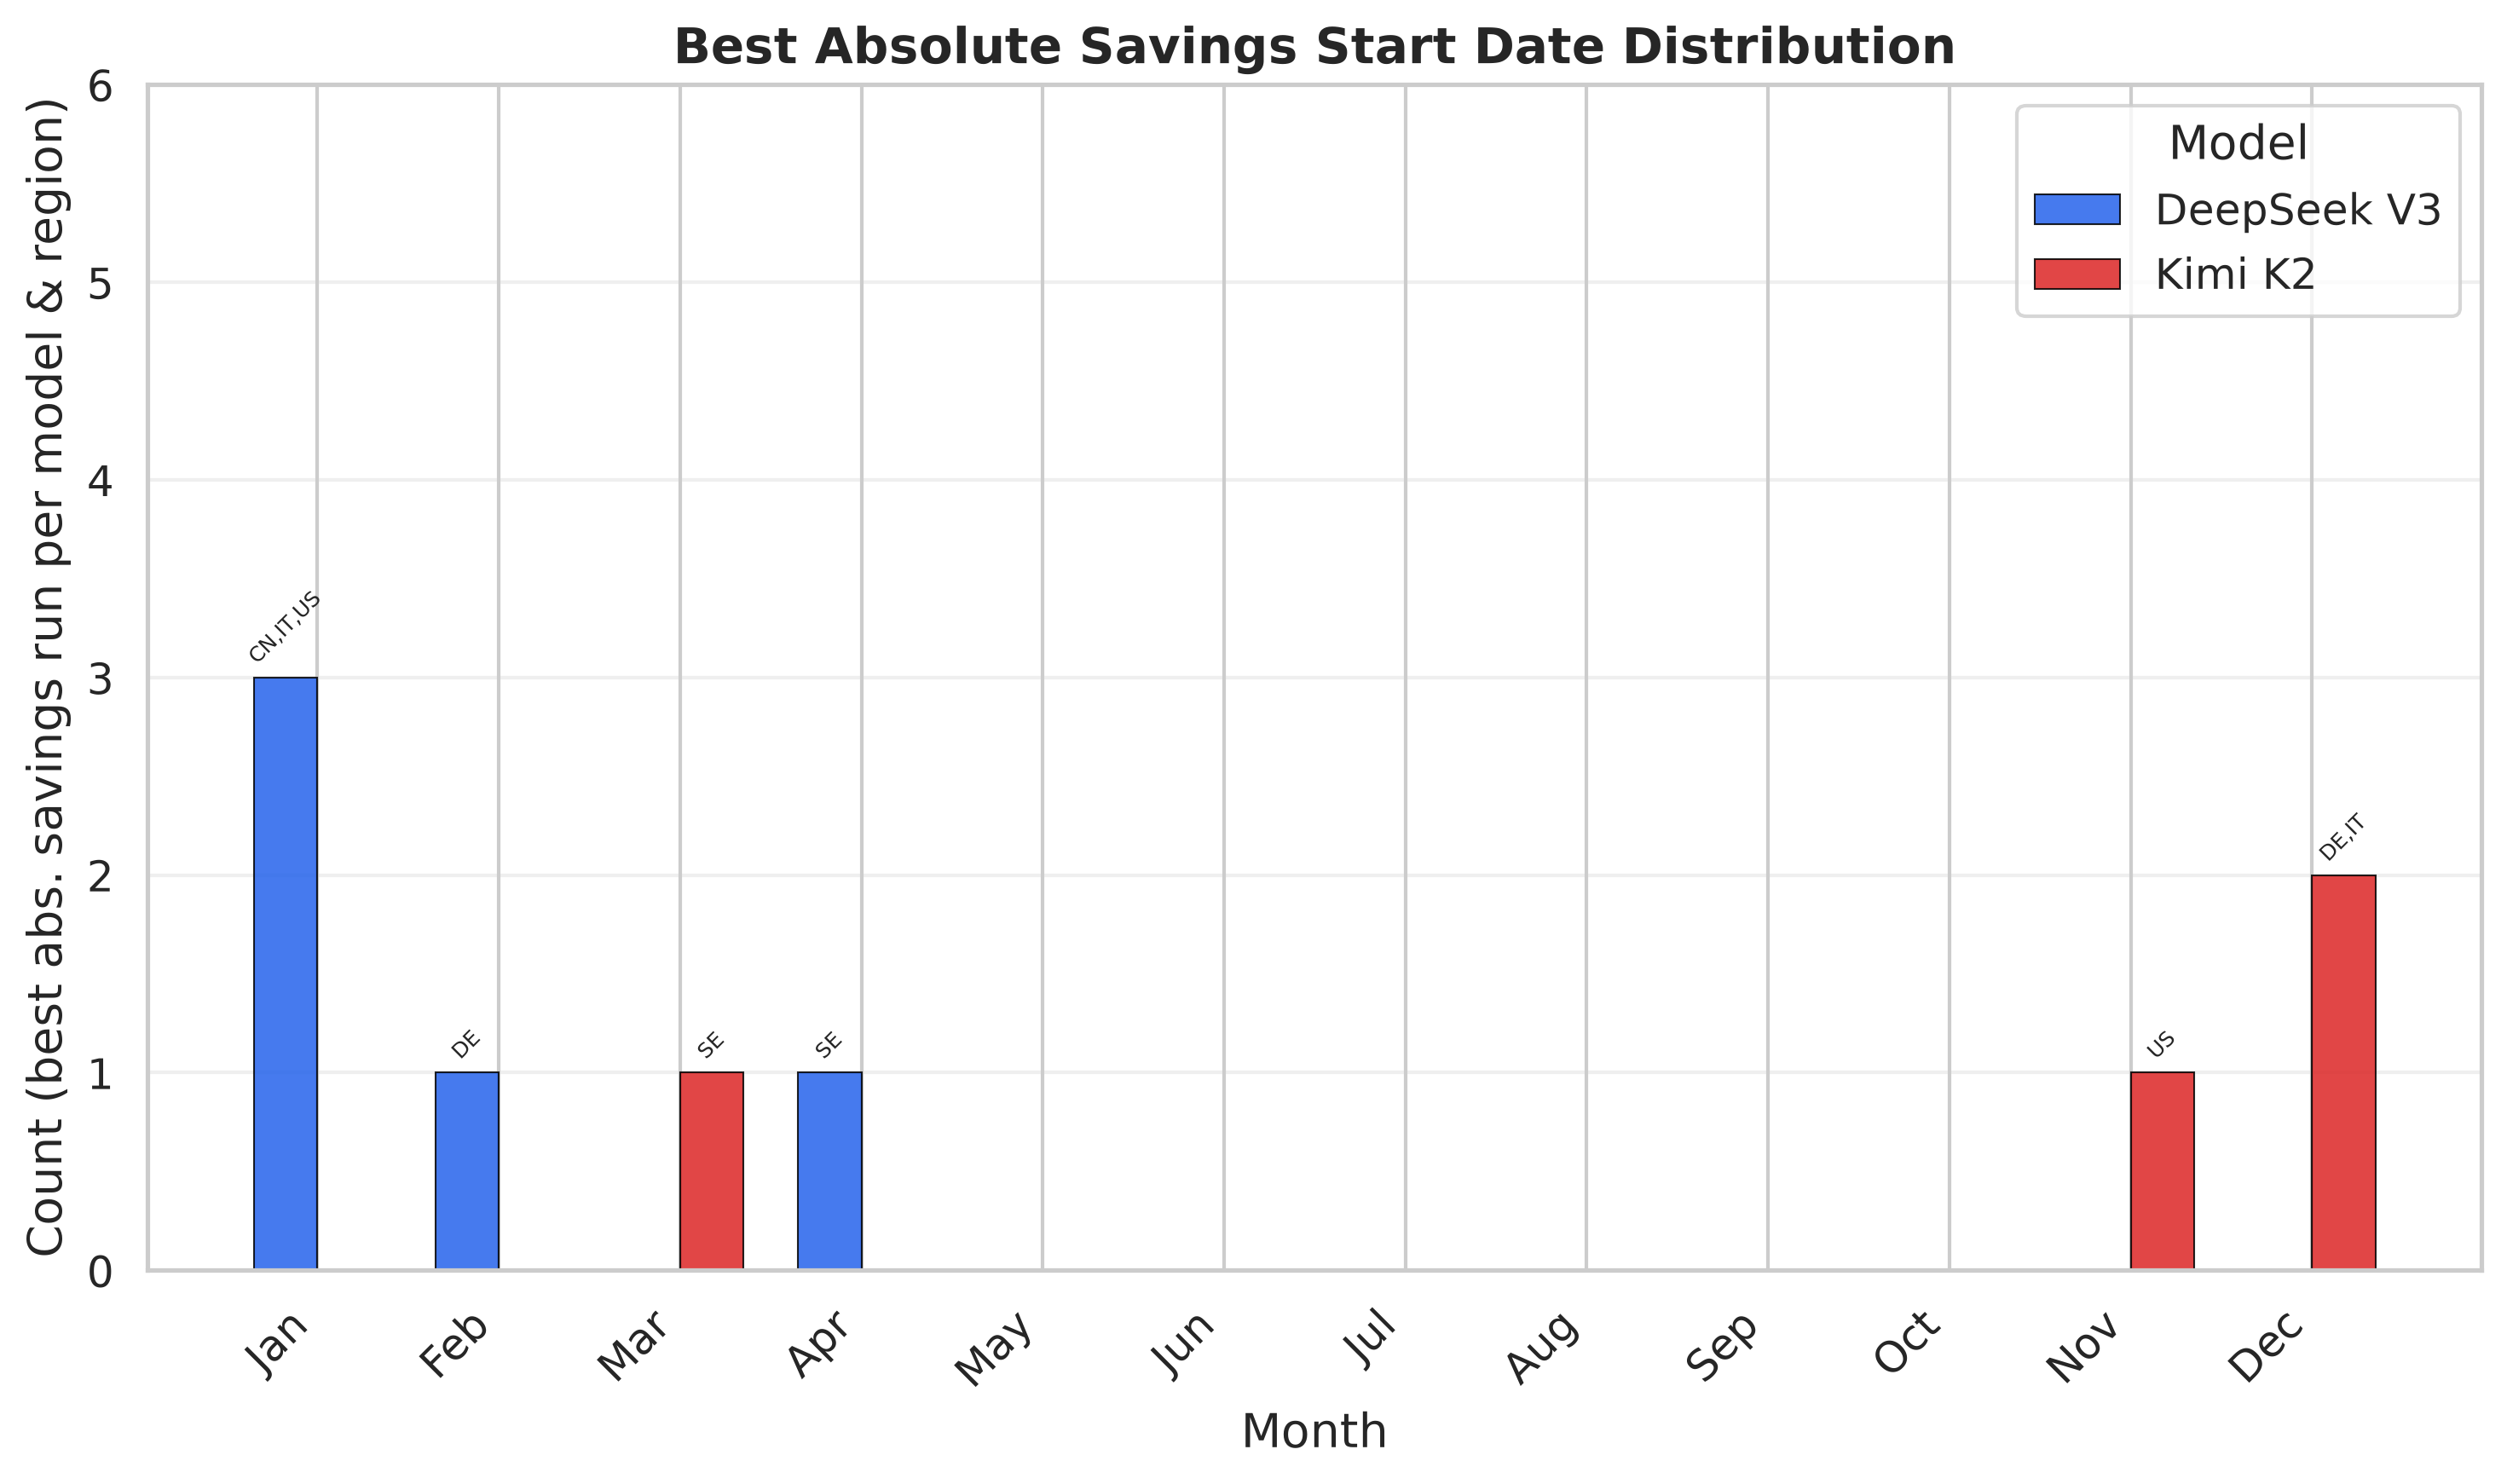
\includegraphics[width=0.95\textwidth,height=0.58\textheight,keepaspectratio]{assets/best_abs_startdate_histogram.png}
    \end{column}
  \end{columns}

  \begin{itemize}
    \item Winter starts (Nov--Feb) consistently outperform summer starts.
    \item Effect is \textbf{secondary} to the hysteresis policy choice.
    \item Difference between best/worst start: $\sim$20pp (IT), $<$2pp (CN).
  \end{itemize}

\end{frame}

